% Data, hierarchy and typology -- budget 850 words (body text).
% Sources: results/paper/tables/Table1_data_inventory.csv, Table2_typology.csv; docs/methods.md section 1;
% docs/results_summary.md; external facts from bensalah2025dib (full text read) and the UCI records.
\section{Data, hierarchy and typology}\label{sec:data}

\subsection{Datasets}\label{sec:datasets}

The study uses the UCI high-resolution load dataset from smart meters in four Moroccan cities \cite{bensalah2025uci,bensalah2025dib}, introduced with a load-forecasting study \cite{bensalah2025opsearch}. The meters are installed by the national utility ONEE on 22~kV distribution feeders and record at 10-min intervals (30~min in Marrakech); the data were exported manually from the meters \cite{bensalah2025dib}. In Laâyoune, Boujdour and Foum El Oued the dataset covers every 22~kV feeder departure \cite{bensalah2025dib}, so each city is observed in full. Each feeder is a \emph{zone} in the dataset's terminology.

Table~\ref{tab:data} lists the series. The three southern cities (15 zones, in amperes) share one 10-min timeline from 14 September 2022 to 24 May 2024, with the same 12 missing time stamps in every zone. We call them the \emph{southern system}; it carries most of the analysis. Marrakech (2 zones, in kW, 2023) is recorded on its own 30-min timeline and is treated as a separate system. The UCI Tetouan dataset \cite{salam2018uci,salam2018irsec}, three distribution networks of one city at 10-min steps in 2017, is used only to test transfer to a new system (Section~\ref{sec:results}). Fig.~\ref{fig:data}(a) locates the five cities.

None of the datasets comes with event labels: there is no record of which zeros or flat stretches are outages and which are acquisition failures. Exact zeros alone occupy 7,201 zone-steps in the southern system (Table~\ref{tab:data}). All time stamps are used as recorded, without any clock correction, so that clock errors remain observable as a data property.

\begin{table}[t]
\centering
\caption{Datasets. Regular steps: length of the regular time grid from the first to the last stamp. Missing steps: grid steps without a record. Zone-steps: one zone at one time step.}
\label{tab:data}
\footnotesize
\setlength{\tabcolsep}{4pt}
\begin{tabularx}{\textwidth}{@{}l c c c Y r r r@{}}
\toprule
City & Zones & Step & Unit & Period & Regular & Missing & Exact-zero \\
     &       & (min) &     &        & steps   & steps   & zone-steps \\
\midrule
Laâyoune     & 5 & 10 & A  & 14 Sep 2022 -- 24 May 2024 & 88,890 & 12 & 1,465 \\
Boujdour     & 3 & 10 & A  & 14 Sep 2022 -- 24 May 2024 & 88,890 & 12 & 1,413 \\
Foum El Oued & 7 & 10 & A  & 14 Sep 2022 -- 24 May 2024 & 88,890 & 12 & 4,323 \\
Marrakech    & 2 & 30 & kW & 9 Jan 2023 -- 8 Jan 2024   & 17,520 & 25 & 101 \\
Tetouan$^{a}$ & 3 & 10 & n.s. & 1 Jan 2017 -- 30 Dec 2017 & 52,416 & 0 & 0 \\
\bottomrule
\end{tabularx}

\vspace{2pt}
\footnotesize{$^{a}$Transfer test only. n.s.: unit not stated in the repository record \cite{salam2018uci}.}
\end{table}

\begin{figure}[t]
\centering
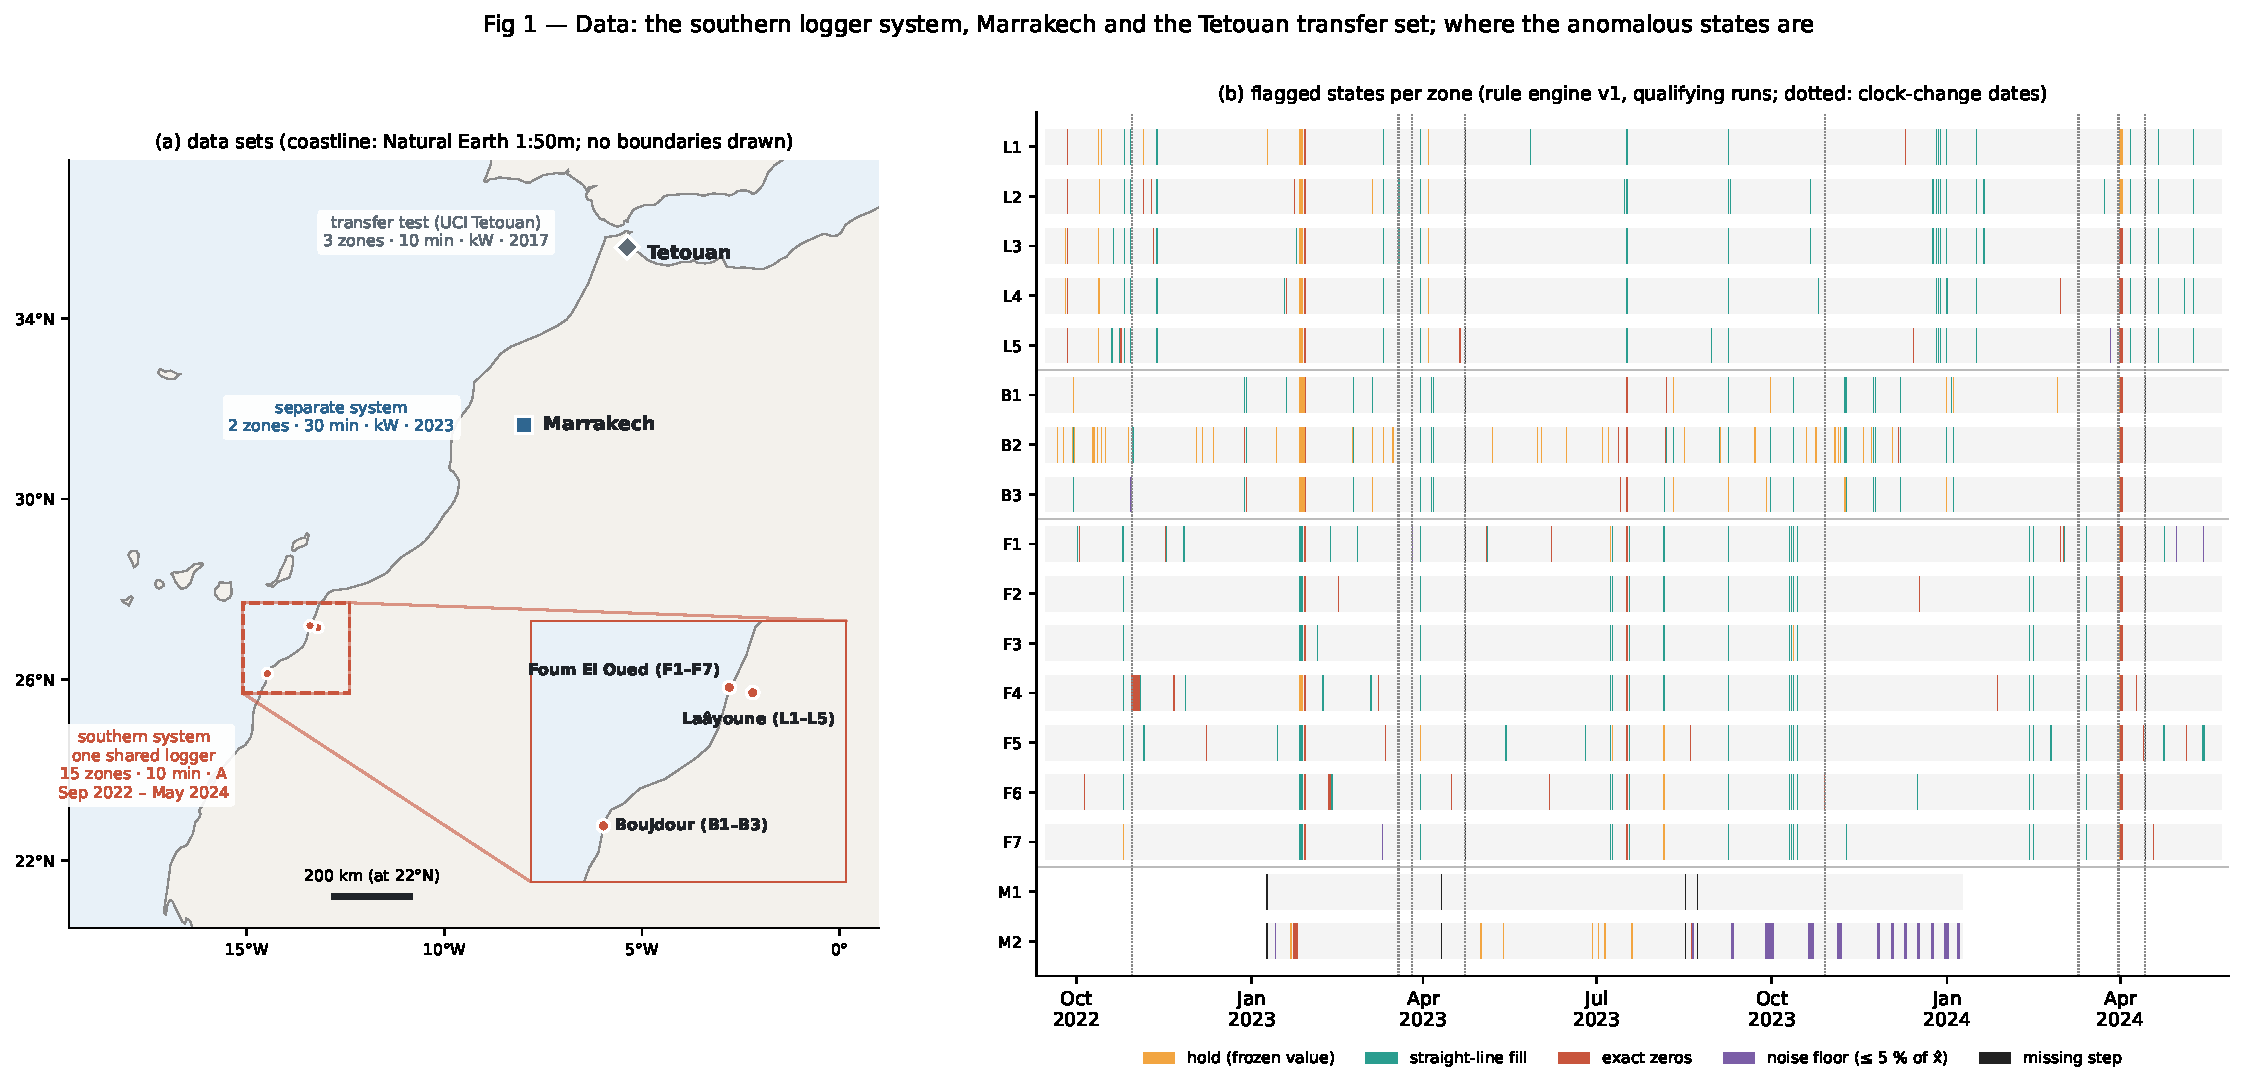
\includegraphics[width=\textwidth]{Figure_1}
\caption{Data. (a) The five cities. Laâyoune, Boujdour and Foum El Oued (15 zones, 10~min, A) share one recording timeline; Marrakech (2 zones, 30~min, kW) is a separate system; Tetouan (3 zones, 2017) is the transfer test. Coastline from Natural Earth (1:50m, public domain); no boundaries are drawn. (b) Anomalous states per zone (holds, straight-line fills, exact zeros and noise-floor runs of qualifying length, and missing steps; Section~\ref{sec:method}); dotted lines mark clock-change dates. Time stamps as recorded.}
\label{fig:data}
\end{figure}

\subsection{The telemetry hierarchy}\label{sec:hierarchy}

The southern series form a three-level hierarchy: zone (one feeder), city (all feeders of one city) and region (the three cities). Each level corresponds to a different cause of a disturbance. A feeder fault or planned maintenance affects one zone. Losing a city's supply point de-energises all of that city's zones while the other cities keep running. A regional event affects several cities at once.

The acquisition chain forms a fourth, non-electrical layer. The three cities are recorded on one timeline, and a failure in the shared recording or export process can hit zones in different cities at the same time step, regardless of the electrical topology. Such a failure also leaves traces that a de-energised feeder does not: series held at an identical value, stretches that are perfectly straight lines, and exact zeros where a de-energised feeder often reads a small, noisy residual current. The method uses these signatures together with the level at which an anomaly appears: simultaneity across cities, combined with these traces, is evidence of an artefact, whereas a noise floor confined to one zone or one city is evidence of a grid event.

\subsection{Problem formulation}\label{sec:problem}

Let $x_{z,t}$ be the recorded value of zone $z$ at time step $t$, and $P$ the number of steps per day (144 at 10~min, 48 at 30~min). The expected value is the median of the same time-of-day slot over the previous $K = 14$ days, excluding zeros:
\begin{equation}
\xh_{z,t} = \operatorname{median}\left\{ x_{z,t-kP} \;:\; k = 1,\dots,K,\; x_{z,t-kP} \neq 0 \right\}.
\label{eq:expected}
\end{equation}
The relative level
\begin{equation}
\rho_{z,t} = x_{z,t}/\xh_{z,t}
\label{eq:rho}
\end{equation}
is unit-free, so amperes, kilowatts and feeders of different sizes are compared on one scale.

An anomalous \emph{item} $i$ is a time span with a set of affected zones. Its type $y_i$ belongs to $\mathcal{Y} = \{\mathrm{A1},\dots,\mathrm{A4},\mathrm{G1},\dots,\mathrm{G5},\mathrm{N}\}$ (Section~\ref{sec:typology}). The task has four parts: \emph{detection}, finding the items; \emph{attribution}, estimating a probability distribution $p_i(y)$ over $\mathcal{Y}$ for each item; \emph{localisation}, identifying the level (zone, city or region) that carries the anomaly; and \emph{type-aware cleaning}, imputing artefacts while keeping grid events in the data and marking them. All four must be solved without labelled examples.

\subsection{Typology}\label{sec:typology}

Table~\ref{tab:typology} and Fig.~\ref{fig:typology} define nine anomaly types, each with a measurable signature at one level of the hierarchy. The four \emph{data artefacts} are zero-fill gaps across cities (A1), simultaneous fills of several zones by held values or straight lines (A2), the same fills in a single zone (A3), and clock errors that shift the daily profile after a clock-change date (A4). The five \emph{grid events} are regional outages (G1), city outages (G2), unplanned feeder outages (G3), planned work (G4) and load transfers between feeders (G5). Items that match no anomalous pattern are labelled normal (N).

Straight-line fills were not part of the initial typology. They appeared in the data audit (Section~\ref{sec:results}) and are now part of A2 and A3. The expected signatures of grid events, in particular gradual restoration and cold-load pick-up after an outage, are hypotheses that Section~\ref{sec:results} tests on the real data.

\begin{table}[t]
\centering
\caption{Typology. Level: the level of the hierarchy at which the signature appears. Rules: the labelling rules that vote for the type (Section~\ref{sec:method}). Real items: rule items assigned the type in the final catalogue of the real data. $\eta$: share of exact zeros in a dead run; $\pi$: restoration overshoot; $\delta^*$: estimated clock offset; $\kappa$: conservation index.}
\label{tab:typology}
\footnotesize
\setlength{\tabcolsep}{4pt}
\begin{tabularx}{\textwidth}{@{}l L{2.1cm} L{1.9cm} Y L{1.6cm} r@{}}
\toprule
Type & Name & Level & Signature & Rules & Real items \\
\midrule
A1 & Zero-fill gap & Region ($\geq 2$ cities) & Exact zeros ($\eta = 1$) in $\geq 2$ cities at once, often after a hold or straight-line fill; returns at once & R1, R3, R4, R21 & 3 \\
A2 & Simultaneous fill & $\geq 2$ zones & $\geq 2$ zones held at identical values or straight-line interpolated over the same span & R2, R19 & 57 \\
A3 & Single-zone fill & Zone & One zone held or straight-line interpolated while its neighbours move normally & R12, R20 & 98 \\
A4 & Clock error & System, one day & Daily profile shifted by $\delta^* \approx \pm 60$~min after a clock-change date; duplicated or missing stamps & R13, R14, R15 & 14 \\
\midrule
G1 & Regional outage & Region ($\geq 2$ cities) & Noise floor ($\eta < 0.9$) in $\geq 2$ cities; gradual restoration with cold-load overshoot $\pi \geq 1.15$ & R5, R6, R7 & 0 \\
G2 & City outage & City & All zones of one city at the noise floor while the other cities stay normal & R8 (R5, R6) & 1 \\
G3 & Unplanned feeder outage & Zone & One zone at the noise floor at any hour, possibly for more than 24~h & R9, R11 (R6) & 52 \\
G4 & Planned work & Zone & One zone at the noise floor, starting 06:00--11:59, shorter than 6~h & R10 & 70 \\
G5 & Load transfer & $\geq 2$ zones of a city & One zone steps down while another steps up by the same amount ($\kappa \approx 0$) & R16 & 1 \\
\bottomrule
\end{tabularx}
\end{table}

\begin{figure}[t]
\centering
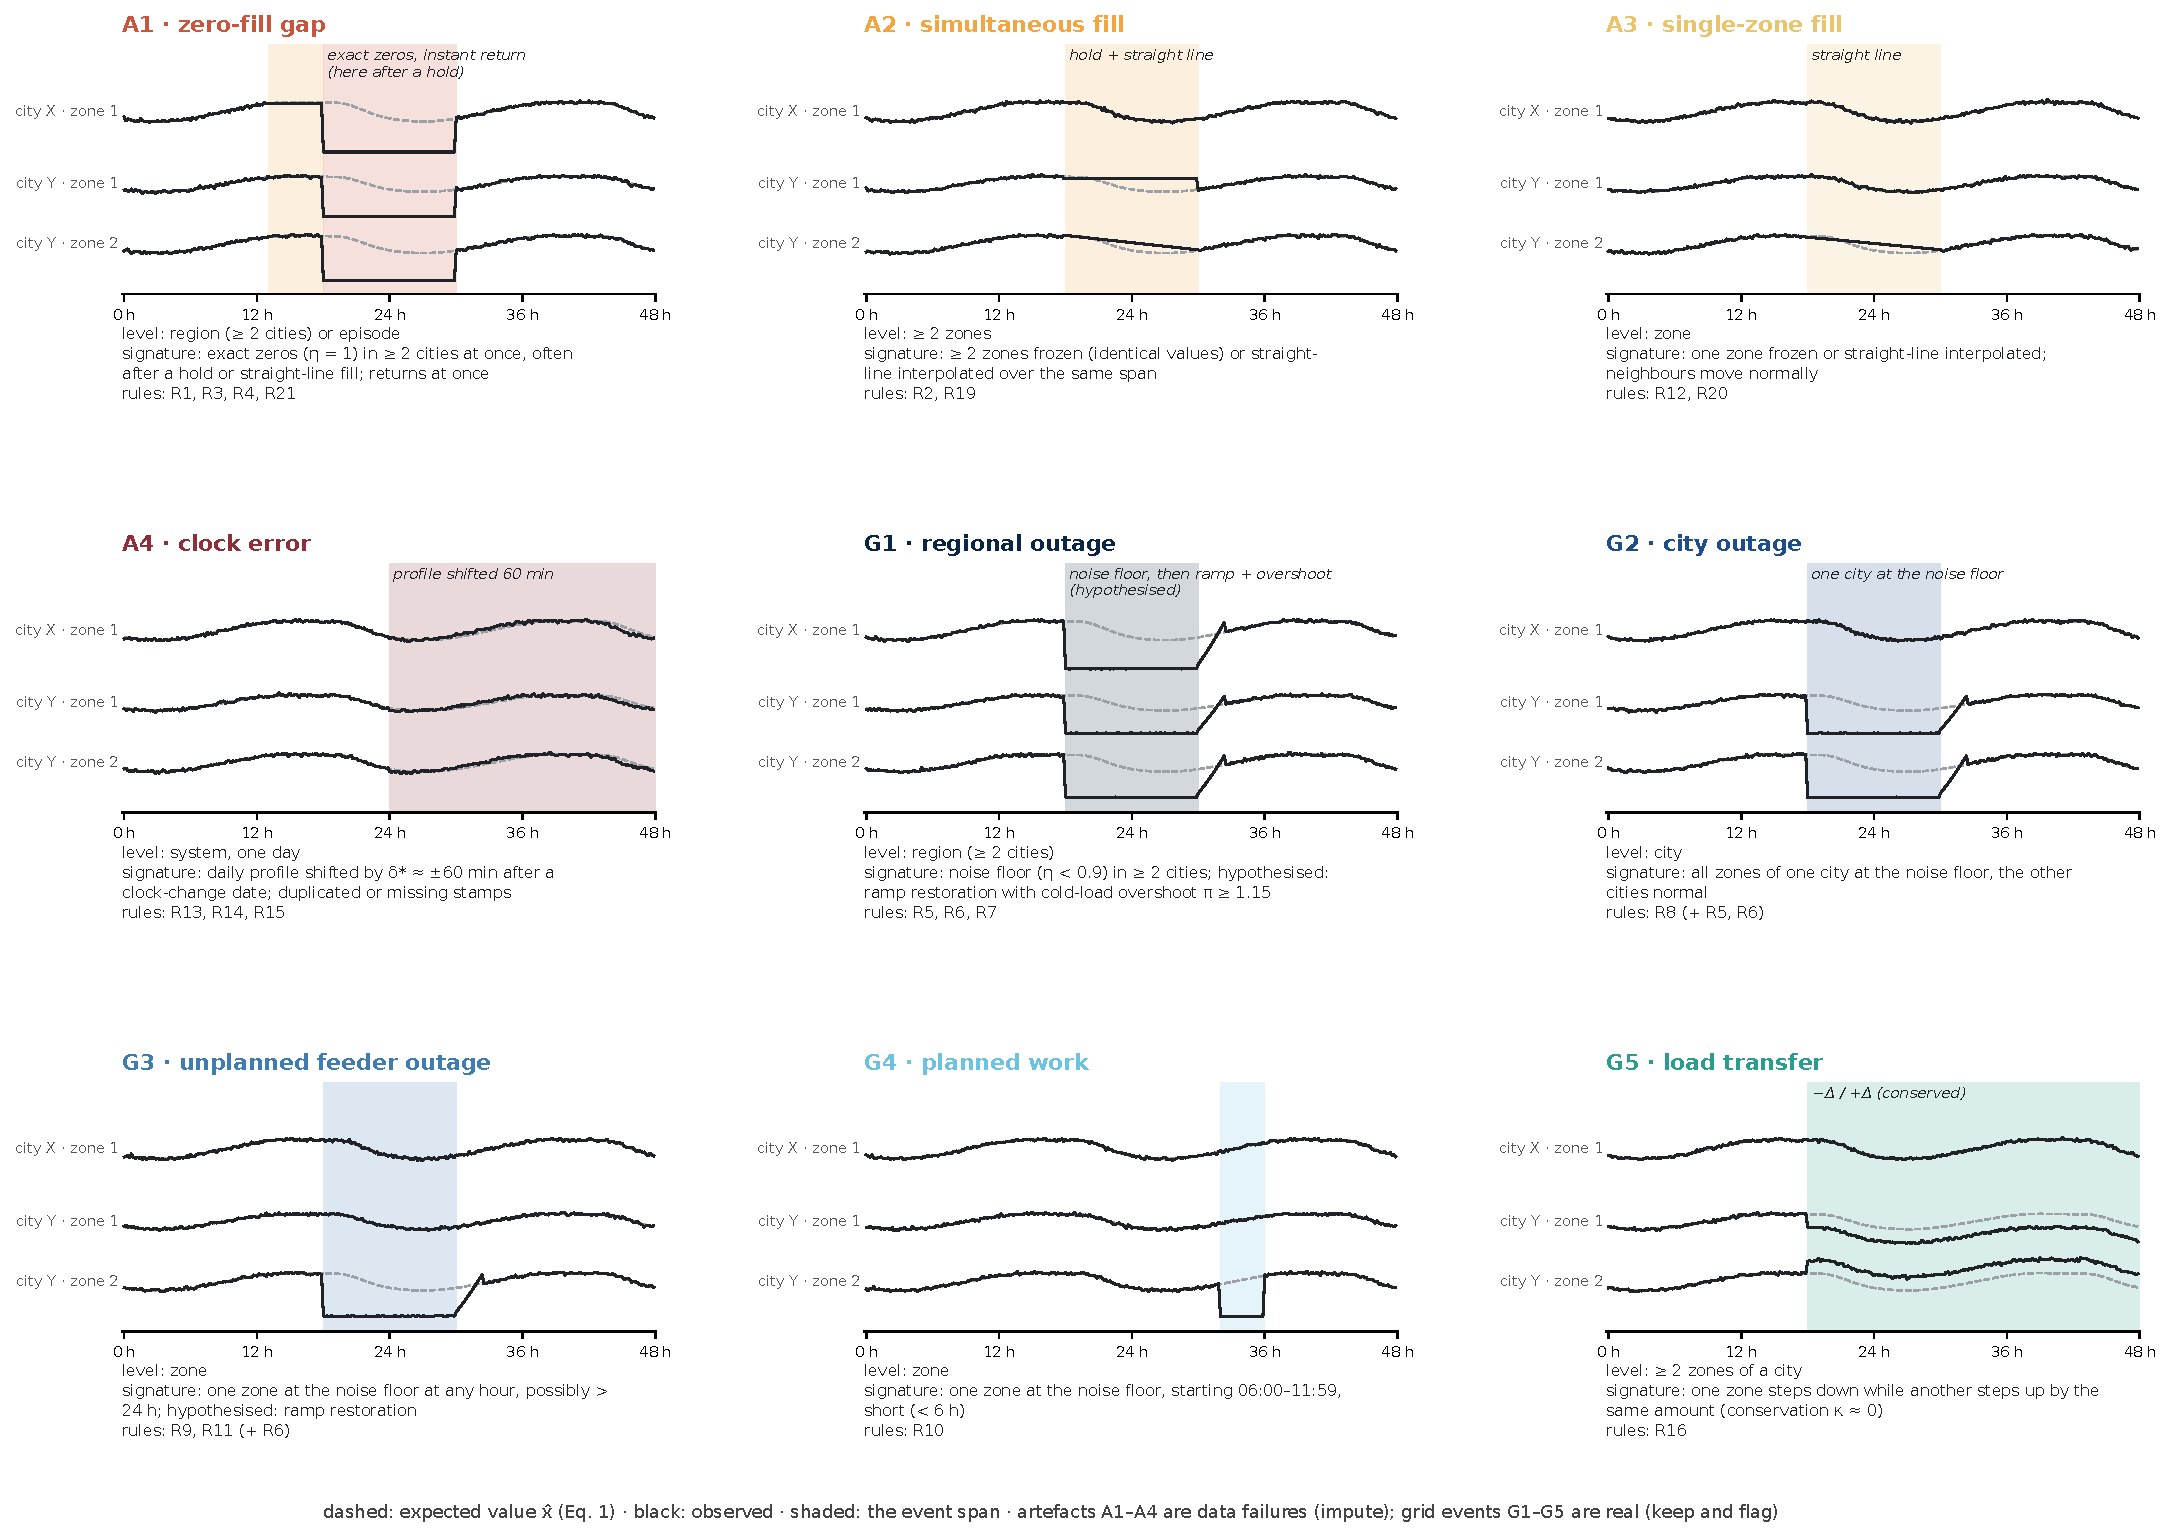
\includegraphics[width=\textwidth]{Figure_2}
\caption{Typology. Four data artefacts (A1--A4) and five grid events (G1--G5), each with a measurable signature at one level of the zone--city--region hierarchy and the rules that vote for it (schematic). Straight-line fills are part of A2 and A3.}
\label{fig:typology}
\end{figure}
